% AUTO-GENERATED from summary.json (3 runs). Do not edit by hand.
\subsection{Quantitative Results}
\begin{table}[!t]
\caption{Task 1: collision-free free posing: mean$\pm$std over seeds (25-episode deterministic eval)}
\label{tab:res-free}
\centering\small
\begin{tabular}{@{}lccc@{}}
\toprule
Method & Success & Time (s) & Pen. (mm) \\
\midrule
PPO & 1.000$\pm$0.000 & 0.31 & 0.02 \\
\bottomrule
\end{tabular}
\end{table}
\begin{table}[!t]
\caption{Task 2: V$\to$OK$\to$OPEN sequencing: mean$\pm$std over seeds (25-episode deterministic eval)}
\label{tab:res-seq}
\centering\small
\begin{tabular}{@{}lccc@{}}
\toprule
Method & Success & Time (s) & Pen. (mm) \\
\midrule
\bottomrule
\end{tabular}
\end{table}
\subsection{Key Findings}
On Task 1, PPO attains the highest deterministic success rate (1.000) with mean arrival 0.31\,s; Fig.~\ref{fig:learn-free}--\ref{fig:safety} report learning curves, sample efficiency, phase decomposition, wall-clock efficiency, and safety penetration.
\begin{figure}[!t]\centering
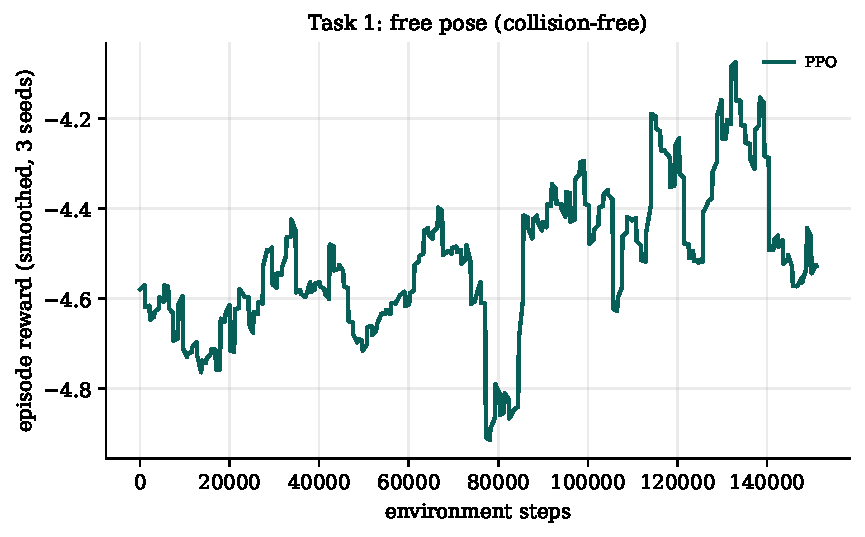
\includegraphics[width=\linewidth]{fig01_learning_free.pdf}
\caption{Task 1 training curves (smoothed success rate vs.\ environment steps; 3 seeds).}\label{fig:learn-free}
\end{figure}

\begin{figure}[!t]\centering
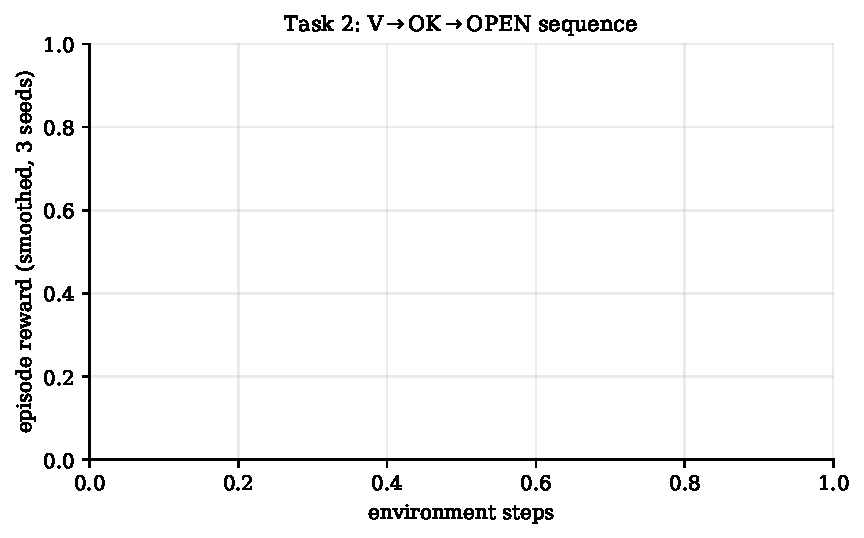
\includegraphics[width=\linewidth]{fig02_learning_seq.pdf}
\caption{Task 2 training curves.}\label{fig:learn-seq}
\end{figure}

\begin{figure}[!t]\centering
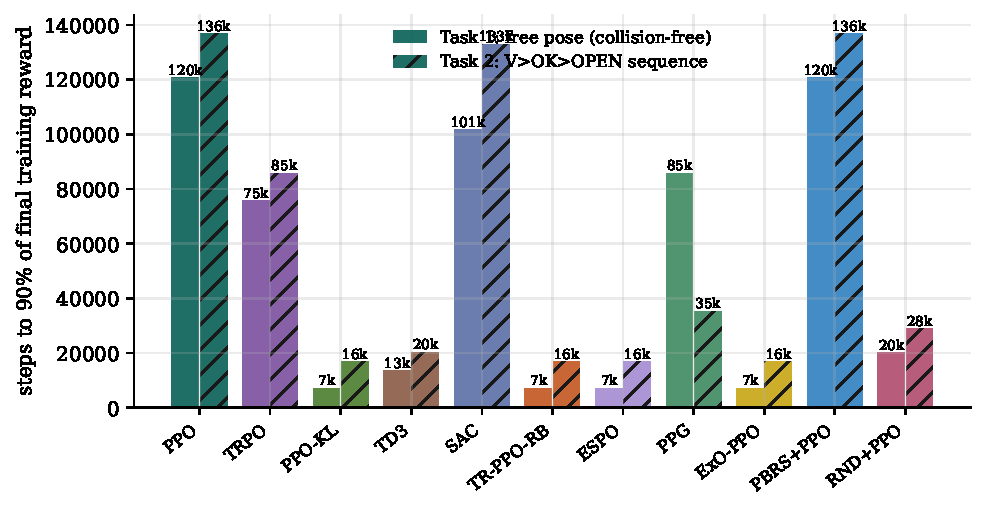
\includegraphics[width=\linewidth]{fig05_sample_efficiency.pdf}
\caption{Sample efficiency: steps for the smoothed training reward to reach 90\% of its final level.}\label{fig:eff}
\end{figure}

\begin{figure}[!t]\centering
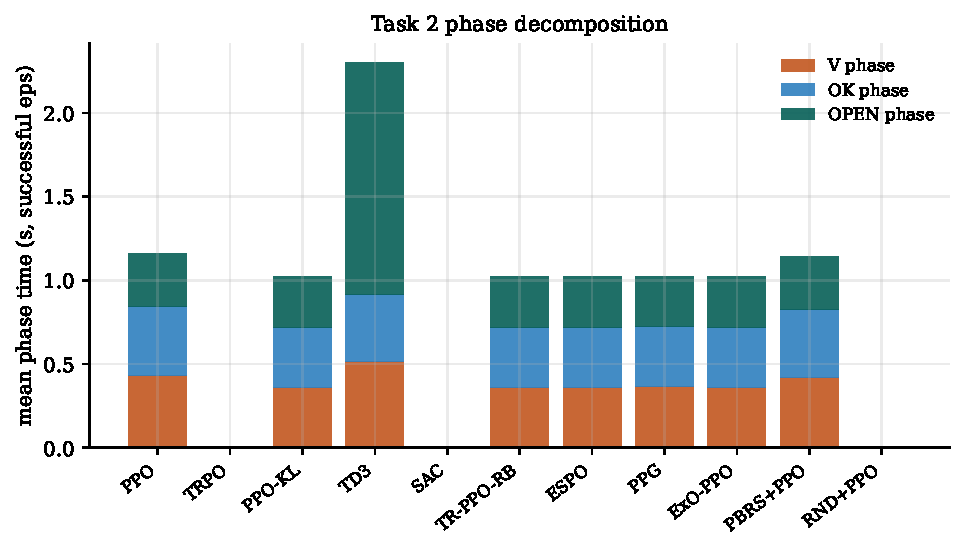
\includegraphics[width=\linewidth]{fig10_phase_decomposition.pdf}
\caption{Task 2 per-phase time decomposition on successful episodes.}\label{fig:phase}
\end{figure}

\begin{figure}[!t]\centering
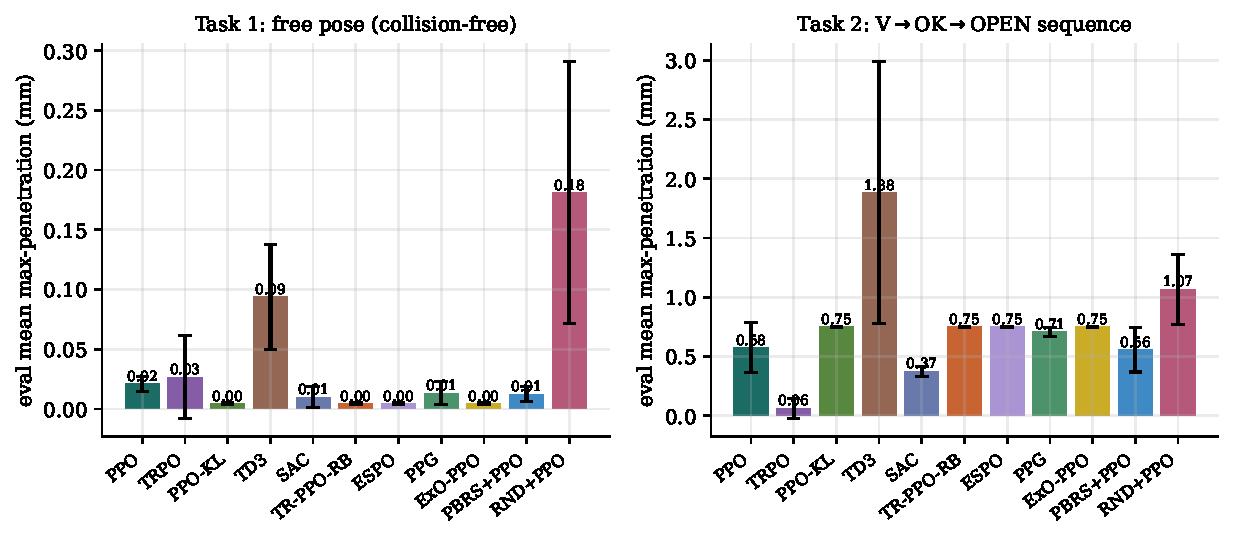
\includegraphics[width=\linewidth]{fig12_safety_penetration.pdf}
\caption{Safety proxy: mean maximum self-penetration during evaluation.}\label{fig:safety}
\end{figure}
